% This is main.tex, uses LLNCS macro package for Springer Computer Science proceedings;
% Version 2.21 of 2022/01/12

%This document contains the structure of the thesis. Here, you can change the section titles and the order of the different sections. The content of the thesis should be added to the different .tex files in the 'Content' folder. References should be added to 'mybibliography.bib'.
%
\documentclass[12pt]{llncs}
%
\usepackage[T1]{fontenc}
% T1 fonts will be used to generate the final print and online PDFs,
% so please use T1 fonts in your manuscript whenever possible.
% Other font encondings may result in incorrect characters.
%
\usepackage{stmaryrd}
\usepackage{graphicx}
\usepackage[export]{adjustbox}
\usepackage{algorithm}
\usepackage{algpseudocode}
\usepackage{listings}
\lstset{
  language=C,
  basicstyle=\small\ttfamily,
  breaklines=true,
  breakatwhitespace=true
}
\graphicspath{ {./images/} }
% Used for displaying a sample figure. If possible, figure files should
% be included in EPS format.
%
% If you use the hyperref package, please uncomment the following two lines
% to display URLs in blue roman font according to Springer's eBook style:
%\usepackage{color}
%\renewcommand\UrlFont{\color{blue}\rmfamily}
%
\usepackage[percent]{overpic}
% Used for overlaying pictures on title page.

\usepackage[dvipsnames]{xcolor}
% Used to define new colors

\usepackage[nottoc,section]{tocbibind}
\setcounter{tocdepth}{4}
% Used to define table of contents.

\usepackage{geometry}
\geometry{
  textwidth=12.2cm,  % llncs has 12.2cm
  textheight=19.3cm, % llncs has 19.3cm
  centering
}
% Used to define the margins of the pages.

\pagestyle{headings}
% Used for page numbering.

\usepackage{hyperref}
% Used for hyperlinking cross-referenced elements.

\usepackage{amsmath}
\usepackage{amsfonts}
\usepackage{amssymb}
% Used for equations

\begin{document}
%
%Start
\newgeometry{textheight=700pt,top=50pt,left=50pt,right=50pt}
\begin{titlepage}
%\vspace*{0.8cm}
\begin{figure}[h]{%
      
\includegraphics[width=0.5\textwidth]{Figures/logo.png}
    }
\end{figure}

\vspace*{2cm}

{\Huge  \textbf{Real-time 2nd order Adaptive Notch Filter Design}}

%\vspace*{6.5cm}
{\raggedleft\vfill{%

%
% ---- Write your names here ----
%
% In case of groups of two students:
% 1. Change \begin{tabular}{c c c} to \begin{tabular}{c c}
% 2. Delete  & {\Large Name 3}
% 3. Delete  & {Student number 3} 
\setlength{\tabcolsep}{12pt} 
\begin{tabular}{c c c}
        {\Large Chieh Fei (Jeffee) Hsiung}  &  {\Large Wentai Ye}  \\
        {R0819932}  & {R0913213}
\end{tabular}
\linebreak
\vspace*{1.5cm}


\textbf{{\large Lab report of course}} \linebreak

%!!!IMPORTANT!!!:
%indicate the appropriate title of your master and major. Check the website https://feb.kuleuven.be/studentenportaal/contact/masterproef-leuven
{\large Signal Processing Algorithms \& Implementations}\linebreak

\textbf{{\large Teaching Asistant:}}  Hannes Rosseel
\linebreak
\textbf{{\large Lecture Professor:}} Dr. Toon van Waterschoot
\linebreak
%\linebreak

\textbf{{\large Academic year:}} {\large 2023-2024}
\linebreak
}\par}

\end{titlepage}
\restoregeometry
\clearpage

%%%%%%%%%%%%%%%%%%%%%%%%%%%%%%%%%%%%%%%%%%%%%%%%%%%%%%%%%%%%%%%%%%%%%%%%%%%%%%%%%%%%%%%%%%%%%%%%%%%% 

\restoregeometry

%
%
% ---- Table of contents ----
%
\tableofcontents

\clearpage

%
% ---- Methodology ----
%
\section{Methodology}
\subsection{Background: Acoustic Feedback}

Acoustic howling is a phenomenon that arises due to an acoustic feedback path, specifically, the occurrence of acoustic coupling between a loudspeaker and a microphone. This coupling results in the microphone picking up the sound signal emitted by the loudspeaker, and subsequently, this captured signal is fed back to the loudspeaker after undergoing amplification. This particular occurrence is commonly referred to as acoustic feedback.

From the perspective of a closed-loop system, the occurrence of howling is contingent upon meeting certain conditions of instability. The analysis of these conditions is rooted in the Nyquist stability criterion, which can be derived from an examination of the closed-loop frequency response of the system illustrated in Figure \ref{fig:system_diagram_original}.

\begin{figure}[ht]
    \centering
    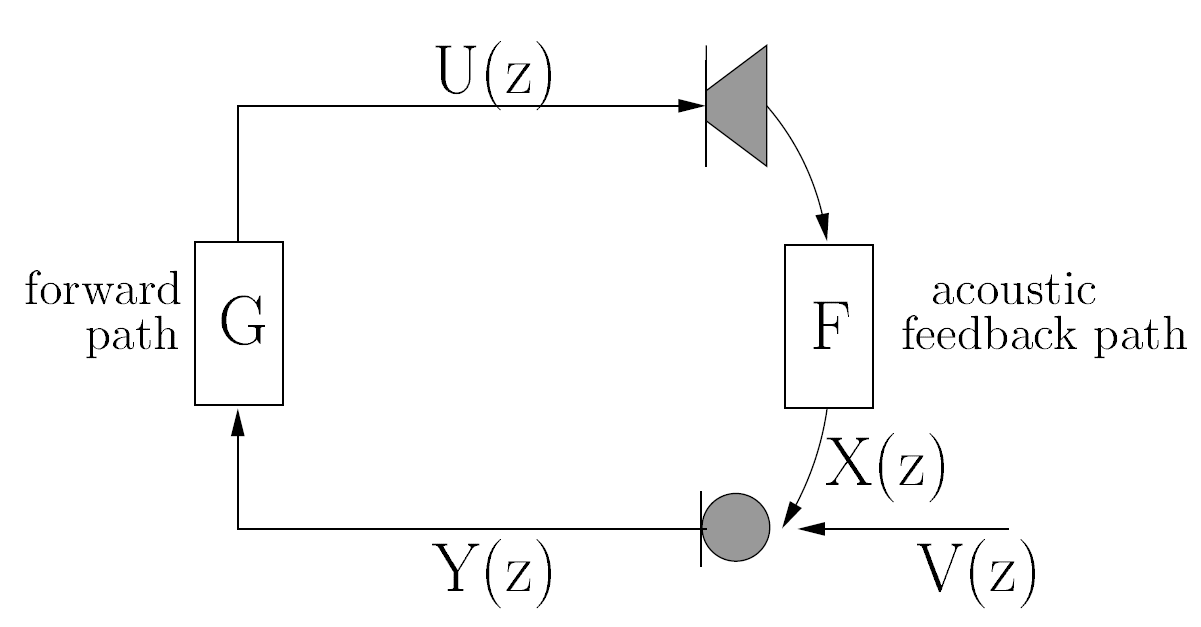
\includegraphics[width=0.8\columnwidth]{images/system_digram_original.png}
    \caption{Acoustic feedback problem in a 1-microphone/1-loudspeaker setup\cite{7077829}}
    \label{fig:system_diagram_original}
\end{figure}

\subsection{Problem statement}
\subsubsection{Assumptions}

For our analysis, we focus on a single-channel setup, consisting of one loudspeaker and one microphone, with the following characteristics:

\begin{itemize}
    \item Linear and flat response in the loudspeaker.
    \item Linear and flat response in the microphone.
    \item Linear and flat response in the forward path (amplifier).
    \item Linear but non-flat response in the acoustic feedback path.
\end{itemize}

The desired system transfer function is:
\begin{equation}
    \frac{U(z)}{V(z)} = G(z)
\end{equation}

The resulting closed-loop system transfer function is:
\begin{equation}
    \frac{U(z)}{V(z)} = \frac{G(z)}{1 - G(z) F(z)}
\end{equation}

This system configuration is prone to spectral coloration, acoustic echoes, and, notably, the risk of instability—our primary concern. The loop response is quantifiable by the loop gain $\mid G(e^{i \omega}) F(e^{i \omega})\mid$ and loop phase $\angle G(e^{i \omega}) F(e^{i \omega})$.

\subsubsection{Nyquist Stability Criterion}:
If a radial frequency $\omega$ exists where

\begin{equation}
    \left\{\begin{array}{l}
    \left|G\left(e^{i \omega}\right) F\left(e^{i \omega}\right)\right| \geq 1 \\
    \angle G\left(e^{i \omega}\right) F\left(e^{i \omega}\right)=n 2 \pi, n \in \mathbb{Z}
    \end{array}\right.
\end{equation}

then the closed-loop system is unstable. Excitation of the unstable system at this critical frequency $\omega$ will result in oscillation at the frequency, known as howling.

An example of closed-loop system instability is depicted in Figure \ref{fig:input_spectrogram}.

\subsubsection{Target}

\begin{figure}[ht]
    \centering
    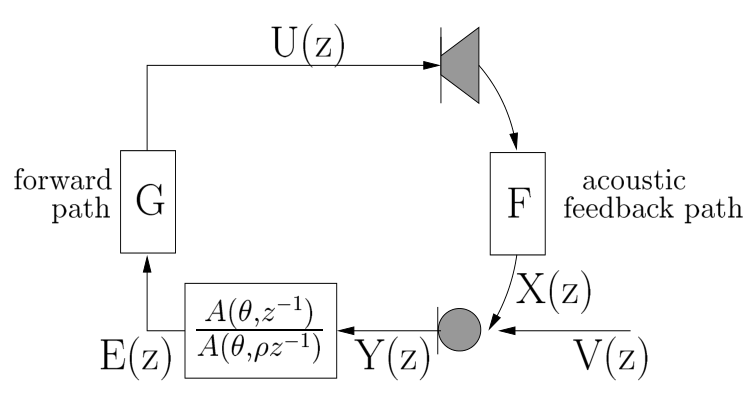
\includegraphics[width=0.8\columnwidth]{images/system_digram_anf.png}
    \caption{Including an adaptive notch filter in the 1-microphone/1-loudspeaker
setup\cite{7077829}}
    \label{fig:system_diagram_anf}
\end{figure}

The primary goal of this project is to remove feedback oscillations in closed-loop systems as shown in Figure \ref{fig:system_diagram_anf}. Our approach involves initially addressing a single narrow-band noise source in a signal using a simplified method with a fixed pole radius, denoted as $\rho$. We then advance this technique by adopting an iteratively adaptive $\rho$, enhancing the filter's effectiveness. 

In our implementation of these filters, we have utilized both C and assembly languages on a C5515 development board. To assess performance in an offline setting, we tested the filters with a specifically generated signal, analyzing the time-spectrum of both the input and the output to evaluate the efficacy of the noise reduction. Additionally, we conducted real-time system testing, where a microphone served as the input and a speaker was used as the output. This setup allowed us to observe the filter's performance in a live audio processing environment, demonstrating its capability to effectively manage feedback oscillations.


\subsection{Adaptive Notch Filtering}
The objective of acoustic feedback control in audio systems is to either completely eliminate acoustic coupling or to partially reduce howling in loudspeaker signals. This can be achieved through manual control techniques such as optimal microphone and loudspeaker placement, pre-emptive room equalization with 1/3 octave graphic EQ filters, and targeted suppression of specific room modes using notch filters. Alternatively, automatic control requires no sound engineer intervention and encompasses various methods: gain reduction for adjusting gain post-howling detection, phase modulation methods for loop gain smoothing, spatial filtering through adaptive microphone beamforming to lessen direct coupling, and room modeling involving adaptive inverse filtering and feedback cancellation. Within these, the gain reduction approach, further classified into automatic gain control, automatic equalization, and notch filtering, is particularly noteworthy for its application in full-band gain reduction and specific frequency band suppression. In this project, we chose gain reduction method by utilizing the adaptive notch filter.

Firstly, let us recall the biquad filter in the $z$-domain without any constraints:
\begin{equation}
    H\left(z^{-1}\right)=\frac{b_o+b_1 z^{-1}+b_2 z^{-2}}{1+a_1 z^{-1}+a_2 z^{-2}}
\end{equation}
which for $b_o=1$, can be expressed in polar coordinates (in the complex plane) in terms of a zero radius, $\zeta$, and zero angle $\omega_z$, and a pole radius, $\rho$, and pole angle, $\omega_p$ as follows
\begin{equation}
    H\left(z^{-1}\right)=\frac{\left(1-\zeta e^{j \omega_z} z^{-1}\right)\left(1-\zeta e^{-j \omega_z} z^{-1}\right)}{\left(1-\rho e^{j \omega_p} z^{-1}\right)\left(1-\rho e^{-j \omega_p} z^{-1}\right)}
\end{equation}

In order to convert this filter into a more suitable form where its coefficients can be adapted, two constraints need to be subsequently introduced.

The first of these constraints is to make the poles and zeros lie on the same radial line, defined by angle $\omega$ in the complex plane (see Fig. 1), i.e. $\omega_z=\omega_p=\omega$. These poles and zeros must also lie completely within the unit circle, where the zeros would be in between the poles and the unit circle in order to define a notch filter. The intuition behind this is that placing a zero near to the unit circle would attenuate all the frequency components in the neighbourhood of the angular frequency, $\omega$, defining that particular radial line. Placing a pole on the same radial line then creates a resonance at $\omega$, with the bandwidth of the notch filter becoming narrower as $\rho \rightarrow \zeta$.

The second constraint on the biquad filter is to let the zeros all lie on the unit circle so that $\zeta=1$. In this case the frequency component at $\omega$ would be completely attenuated and the pole at the same radial line would once again create a resonance at $\omega$, with the bandwidth of the notch filter becoming narrower as $\rho \rightarrow 1$.

Imposing these constraints on the biquad filter of (3), results in the constrained biquad filter:
\begin{equation}
    \begin{aligned}
     H\left(z^{-1}\right) & =\frac{\left(1-e^{j \omega} z^{-1}\right)\left(1-e^{-j \omega} z^{-1}\right)}{\left(1-\rho e^{j \omega} z^{-1}\right)\left(1-\rho e^{-j \omega} z^{-1}\right)} \\
    & =\frac{1-2 \cos (\omega) z^{-1}+z^{-2}}{1-2 \rho \cos (\omega) z^{-1}+\rho^2 z^{-2}} \\
    & =\frac{1-a z^{-1}+z^{-2}}{1-\rho a z^{-1}+\rho^2 z^{-2}}
    \end{aligned}
\end{equation}
where $a \triangleq 2 \cos (\omega)=2 \cos \left(2 \pi f / f_s\right)$ is the only parameter we need to estimate (since it appears in both the numerator and denominator) and is directly related to the centre frequency, $f$, of the notch filter. Consequently, by adapting the $a$ coefficient, the centre frequency of the notch filter also changes resulting in an ANF.\cite{ali2023frequency}

\subsection{ANF-LMS Algorithm}

The second-order constrained Adaptive Notch Filter (ANF) utilizing a Direct-Form II architecture is optimized for memory efficiency, a critical aspect in digital signal processing. This architecture segregates the filter into a feedforward Finite Impulse Response (FIR) section and a feedback Infinite Impulse Response (IIR) section. Specifically designed to target and diminish certain frequencies, such as those contributing to acoustic feedback, the filter adapts its coefficients in response to signal variations. The adaptation is achieved by updating the FIR coefficients according to the input signal and a chosen algorithm like LMS, then reflecting these changes in the IIR section. This mirroring ensures that the filter consistently suppresses the intended frequencies and remains stable, even when the characteristics of the noise or feedback evolve over time. This method not only streamlines the adaptation process but also enhances the filter's stability in dynamic acoustic environments.

The Least Mean Squares (LMS) algorithm is used for the coefficient update\cite{vanwaterschoot2014}, ensuring efficient and effective adaptation to the changing acoustic environment. It adapts over time by adjusting its parameters to minimize the difference between the filtered and actual signals. The algorithm inputs include the step size $μ$, which affects convergence speed; initial and final pole radii $\rho(0)$ and $\rho(\infty)$, which determine the notch filter's initial width and its convergence target; the decay time constant $\lambda$, guiding the rate at which $\rho(t)$ approaches $\rho(\infty)$; and the input signal $y(t)$. The output $x(t)$ is the filtered signal, and $a(t)$ represents the adaptive filter coefficients. At each iteration $t$, the algorithm updates the pole radius $\rho(t)$, computes the current filtered output $x(t)$, calculates the error $e(t)$ between the filtered and actual signals, and then adjusts the filter coefficients $a(t)$ to reduce this error, iteratively optimizing the filter's performance to suppress the noise.

\begin{algorithm}
\caption{2$^{\text{nd}}$ order ANF-LMS algorithm}
\begin{algorithmic}[1]
\State \textbf{Input:} step size $\mu$, initial pole radius $\rho(0)$, final pole radius $\rho(\infty)$, exponential decay time constant $\lambda$, input data $\{y(t)\}_{t=1}^N$, initial conditions $x(0), x(-1), a(0)$
\State \textbf{Output:} 2$^{\text{nd}}$ order ANF parameter $\{a(t)\}_{t=1}^N$
\For{$t = 1, \ldots, N$}
    \State $\rho(t) = \lambda \rho(t - 1) + (1 - \lambda) \rho(\infty)$
    \State $x(t) = y(t) + \rho(t) a(t - 1) x(t - 1) - \rho^2(t) x(t - 2)$
    \State $e(t) = x(t) - a(t - 1) x(t - 1) + x(t - 2)$
    \State $a(t) = a(t - 1) + 2 \mu e(t) x(t - 1)$
\EndFor
\end{algorithmic}
\end{algorithm}




\clearpage

%
% ---- Implementation ----
%
\section{Implementation}
 \subsection{Constraints}
To ensure an IIR filter stability, the design of the filter adheres to two key constraints identified in \cite{vanwaterschoot2014}. The first constraint mandates that the poles and zeros should be aligned on identical radial lines in z-plane. The second constraint requires that both poles and zeros reside within the unit circle, with zeros positioned between the adjacent poles.

These constraint can be mathematically interpreted in the context of filter design. A zero positioned close to the unit circle, denoted as $z_{i}=$ $r_{i} e^{j \omega_{i}}$, with $r_{i}$ approaching unity, effectively attenuates frequencies in close proximity to $\omega_{i}$. Conversely, a pole is situated on the same radial line, represented as $p_{i}=\alpha r_{i} e^{j \omega_{i}}$, introduces a resonant effect at $\omega_{i}$ that  serves to narrow the notch's bandwidth. 

\subsection{Q Format}\label{q_format}
The Q format is a fixed-point number representation commonly used in DSP to enable efficient arithmetic operations on fractional numbers under limited resources. 

A Q format number is represented by notation $Q_{m.n}$, denoting a fixed-point format with 'm' integer bits and 'n' fractional bits. For instance, the specification Q2.14, describes a signed binary fixed-point number with a 16-bits in total, comprising the sign bit, one bit for the integer part, and 14 bits that are the fraction. Namely, a 16-bit signed, or two's complement, integer, is implicitly multiplied by the scaling factor $2^{-14}$.

While the TMS320C5515 DSP board supports arithmetic in 16-bit and 32-bit fixed-point formats, the constraints of register width invariably impose a ceiling on precision that it is inherently limited to 16-bit precision.

Given the ranges of variables empirically observed in the input signal, the corresponding Q formats that represent these values without overflow and with sufficient precision are as follows:

\begin{itemize}
    \item \textbf{Variable $e$} with range \([-0.7970, 0.6775]\), indicated as a signed short which magnitude never exceed unity, is allocated a 16q15 format.
    \item \textbf{Variable $s$} with range \([-4.7065, 4.7443]\), represented a signed short with absolute values under five, is aptly depicted in a 16q11 format, reserving one bit for the sign and four for the integer.
    \item \textbf{Variable $a$} within \([0.9999, 1.9131]\), exhibiting a positive range with an upper limit below two, is expressed as an unsigned short in 16q15 format.
\end{itemize}

With particular attention to the input frequency response at narrow bands of $400Hz$ and $1200Hz$, the following Q formats were found suitable:

\begin{itemize}
    \item \textbf{Variable $\rho$} consistently remains below one and is non-negative, warranting a 16q16 format, fully fractional, represented as an unsigned short.
    \item \textbf{Variable $\mu$}, as predetermined, is in a 16q15 format.
    \item \textbf{Variable $\lambda$} presents a non-negative range capped at maximum one, adhering to a 16q15 format.
\end{itemize}

\subsection{Adaptive Notch Filter Implementation}
The implementation of the Adaptive Notch Filter (ANF) using the Least Mean Squares (LMS) algorithm is encapsulated within a single function. This function is responsible for dynamically adjusting the filter coefficients to minimize the error between the desired and actual filter outputs.

\subsubsection{Function Description}
The ANF function takes as input the current sample of the signal, a pointer to a state buffer that retains the last three samples, a pointer to the adaptive filter coefficient, a pointer to the current and asymptotic values of the bandwidth adjustment parameter $\rho$, and a pointer to the current index in the circular buffer. It returns the filtered signal sample.

% Derived from \autoref{q_format}, the filter is designated with input parameters as outline in \autoref{fig:input_params}.

% \begin{figure}
%     \centering
%     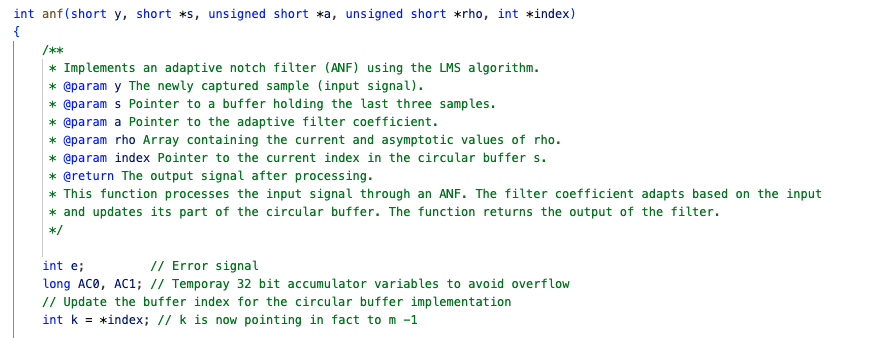
\includegraphics[width=0.7\linewidth]{images/c_code_input_param.png}
%     \caption{Input parameters type of ANF function in C}
%     \label{fig:input_params}
% \end{figure}

Derived from \autoref{q_format}, the filter is designated with input parameters as below:
\begin{lstlisting}[language=C, basicstyle=\small]
int anf(short y, short *s, unsigned short *a, unsigned short *rho, int *index)
{
    /**
     * Implements an adaptive notch filter (ANF) using the LMS algorithm.
     * @param y The newly captured sample (input signal).
     * @param s Pointer to a buffer holding the last three samples.
     * @param a Pointer to the adaptive filter coefficient.
     * @param rho Array containing the current and asymptotic values of rho.
     * @param index Pointer to the current index in the circular buffer s.
     * @return The output signal after processing.
     */
     ......
}
\end{lstlisting}

The data type $short$ of the newly captured sample $y$ is identical to the one of samples stored in the data buffer $s$. $Index$ pointer having $int$ data type to allow for positive and negative indexing in the circular buffer. In the perspective of filter, $a$, the adaptive coefficient, and $\rho$, ratio for adjusting bandwidth configuration embedded within $pole$ and $zero$, are of type $unsigned\ short$.  

\subsubsection{Algorithm Steps}
The function performs the following steps in the ANF-LMS algorithm:

\begin{enumerate}
    \item It calculates the new value of $\rho(m)$, which is a weighted average of its previous value and the asymptotic value, using the coefficients $\lambda$ and $1 - \lambda$. This step ensures that the filter's bandwidth can adapt over time.
    
    \item The state buffer $s$ is updated to reflect the newest sample. This buffer operates in a circular fashion, using the modulo operation to maintain a fixed-size history of the samples.
    
    \item The error signal $e(m)$ is computed, incorporated with latest computed $s(m)$, representing the difference between the desired signal and the filter's output. This error is then used to update the adaptive filter coefficient.
    
    \item Finally, the adaptive filter coefficient $a(m)$ is adjusted based on the error signal and the learning rate $\mu$. This coefficient determines the notch's depth and width, allowing the filter to suppress the undesired frequencies effectively.
\end{enumerate}

The program makes use of 32-bit accumulators to prevent overflow during intermediate calculations. The function also includes a check to constrain the adaptive filter coefficient that $\left\lvert (a(m)) \right\rvert < 2 $, ensuring the stability of the filter.

\subsubsection{Q-format alignment} 
While variables consists of varied Q-format, Q-format alignment prior to blocks of additions and multiplications are required. In our DSP implementation, Q format alignment is exemplified especially during the computation of signal processing terms. Consider the calculating of first term of $s(m)$, which involves the product of $rho(m)$, $a(m-1)$, and $s(m-1)$. Here $\rho[0]$ represented in $Q16$ format, is multiplied by $a[k]$ in $16q15$ format, yielding an intermediate result in $32q31$. This results is then rounded and normalized back to $16q15$ format by right-shifting the accumulator $ACO$, which aligns the Q format for the subsequent multiplication with $s[k]$ in $16q11$ format. The final shift of $ACO$ by $A-Q-FORMAT$ bits ensures that the result is in the desired $16q11$ format, ready to be integrated into $s(m)$.

\begin{lstlisting}[language=C, basicstyle=\small]
// Calculate the first term of s[m]: rho(m) * a(m - 1) * s(m - 1) with k = (m - 1)
AC0 = (long)rho[0] * a[k]; // 16q16 * 16q15 = 32q31
AC0 += 0x4000;             // Add half (since we are shifting 15 bits) to round
AC0 >>= RHO_Q_FORMAT;      // Now AC0 is 32q15
AC0 *= s[k];               // 32q15 * 16q11 (assuming s is in q15 format) = 32q26
AC0 >>= A_Q_FORMAT;        // Normalize to 32q11
\end{lstlisting}

\subsubsection{Circular Buffer Mechanism}
The circular buffer is a key component for implementing the IIR filter, as it allows for efficient memory usage by reusing buffer positions rather than sequentially updating each indexed content, storing the history of samples. The index and k management ensures that the oldest sample is overwritten with the newest one, and that when the function call is finished, the index points to the latest processed index which will be used as the $m-1$ in the next function call.

\subsubsection{Coefficient Adaptation}
The adaptive nature of the filter is realized through the constant update of the coefficient $a(m)$, which is influenced by the error signal and she historical samples. The LMS algorithm ensures that the coefficient converges to a value that minimizes the error signal over time, thereby nullifying the effect of the undesired frequencies.

\subsubsection{Stability and Convergence}
To maintain the stability of the filter, the function includes bounds checking for the coefficient values to not exceed $0x7FFF$, which is two in $16q15$ foramt. Additionally, the shift operations are carefully managed to maintain the fixed-point precision defined by the Q format.

\subsection{Input Parameter Storage register}
The capability of TMS320C5515 registers were studied for effective variables memory manipulation, which is especially critical in assembly programming. As the variables pass from the main script consist of one $short \ y$ where the remaining parameters are of pointers to variables such as $short*$ or $unsigned short*$, registers hypothesized to stored/point to the inputs params are correspondingly $T0$, $AR0$, $AR1$, $AR2$, $AR3$, and return $short\ e$ again in $T0$. The auxilary register were employed given that the specific input parameters are of pointer type that requires manipulation in address phase, which often combined with 23-bit $XARx$ for address and data operations.





\clearpage

%
% ---- Results ----
%
\section{Results}
\subsection{Evaluation Metrics}

\subsubsection{Spectrogram Analysis}
The spectrogram, a time-varying frequency spectrum representation of the signal, will be utilized for functional testing. It visually depicts how the signal's frequency content evolves over time, providing insights into the effects of filtering processes.

\subsubsection{Computational Cost}
Additionally, the computational cost will be assessed in terms of \textbf{required clock cycles}, a metric used in \cite{van2012time}. This measure helps in understanding the efficiency and feasibility of the filter implementation in real-time systems.

\subsection{Functional tests}
The test signal contains narrow bands at 400 and 1200 Hz, superimposed with noise. Its spectrogram (\autoref{fig:input_spectrogram}) serves as a baseline to evaluate the filter's dynamic behavior.

The spectrogram reveals two distinct bands, corresponding to 400 Hz and 1200 Hz. A successful adaptive notch filter (ANF) should show these frequencies attenuated or eliminated, indicating effective removal of target frequencies from the noisy signal.

Our second-order ANF implemented in TMS320C5515 assembly shows this effectiveness. In \autoref{fig:adaptive_assy_spectrogram_l9}, the narrow bands at 400 Hz and 1200 Hz are removed, demonstrating the filter's efficacy.  Here, $\lambda$ is set to 0.9 to focus on the  adapted $\rho(m-1)$ over the infinite $\rho$

\begin{figure}[ht]
    \centering
    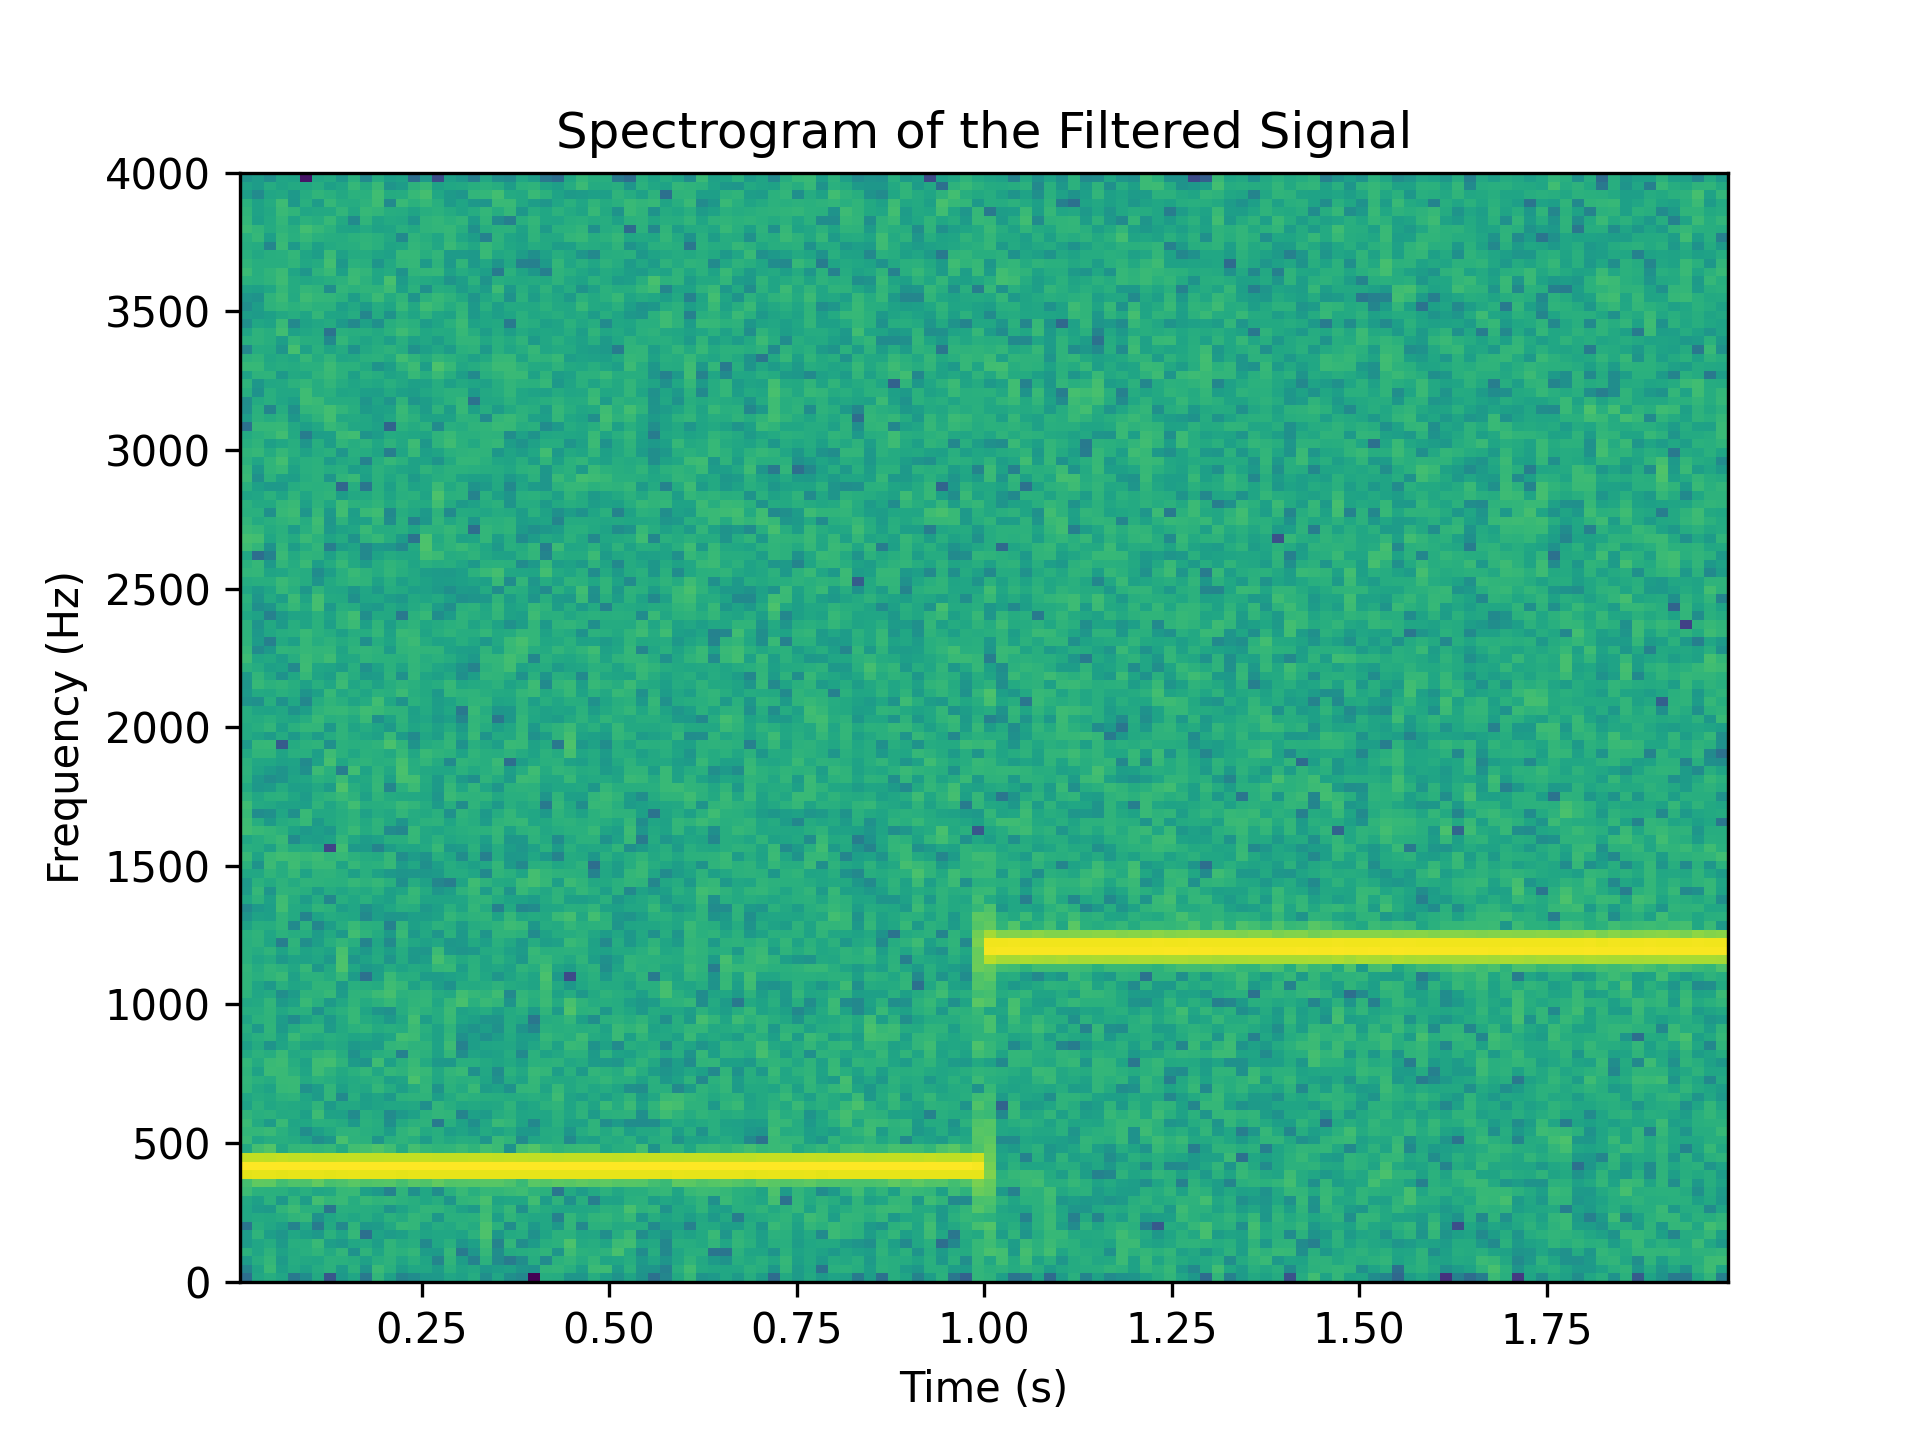
\includegraphics[width=0.5\columnwidth]{images/spectrogram_input.png}
    \caption{Spectrogram of input signal}
    \label{fig:input_spectrogram}
\end{figure}

\begin{figure}[ht]
    \centering
    % First figure
    \begin{minipage}{0.475\columnwidth}
        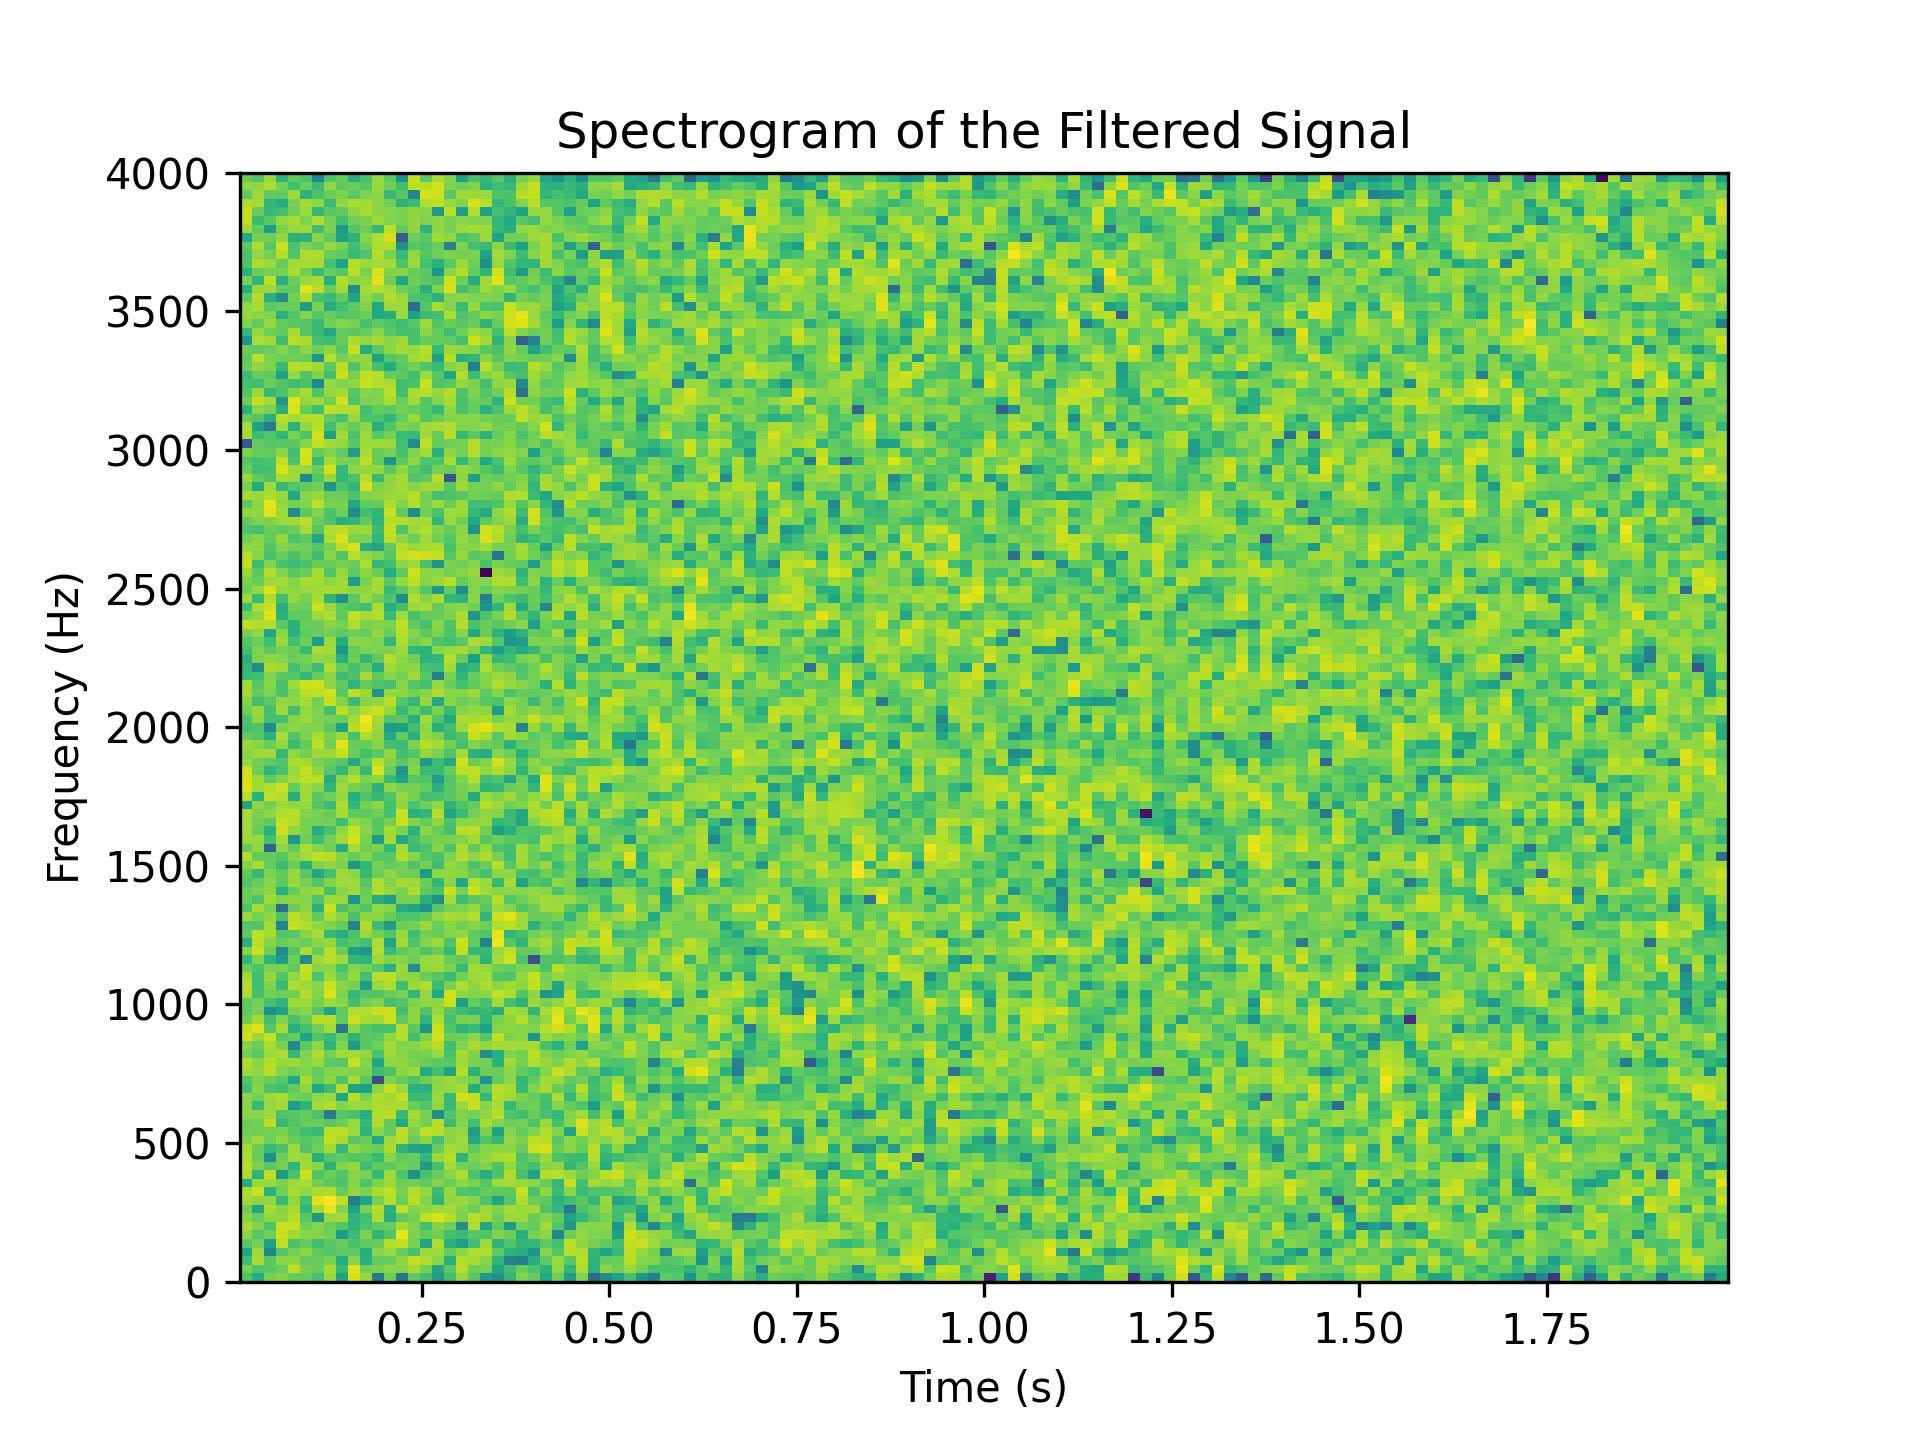
\includegraphics[width=\linewidth]{images/spectrogram_output_a_9.png}
        \label{fig:adaptive_assy_spectrogram_l9}
    \end{minipage}\hfill
    % Second figure
    \begin{minipage}{0.475\columnwidth}
        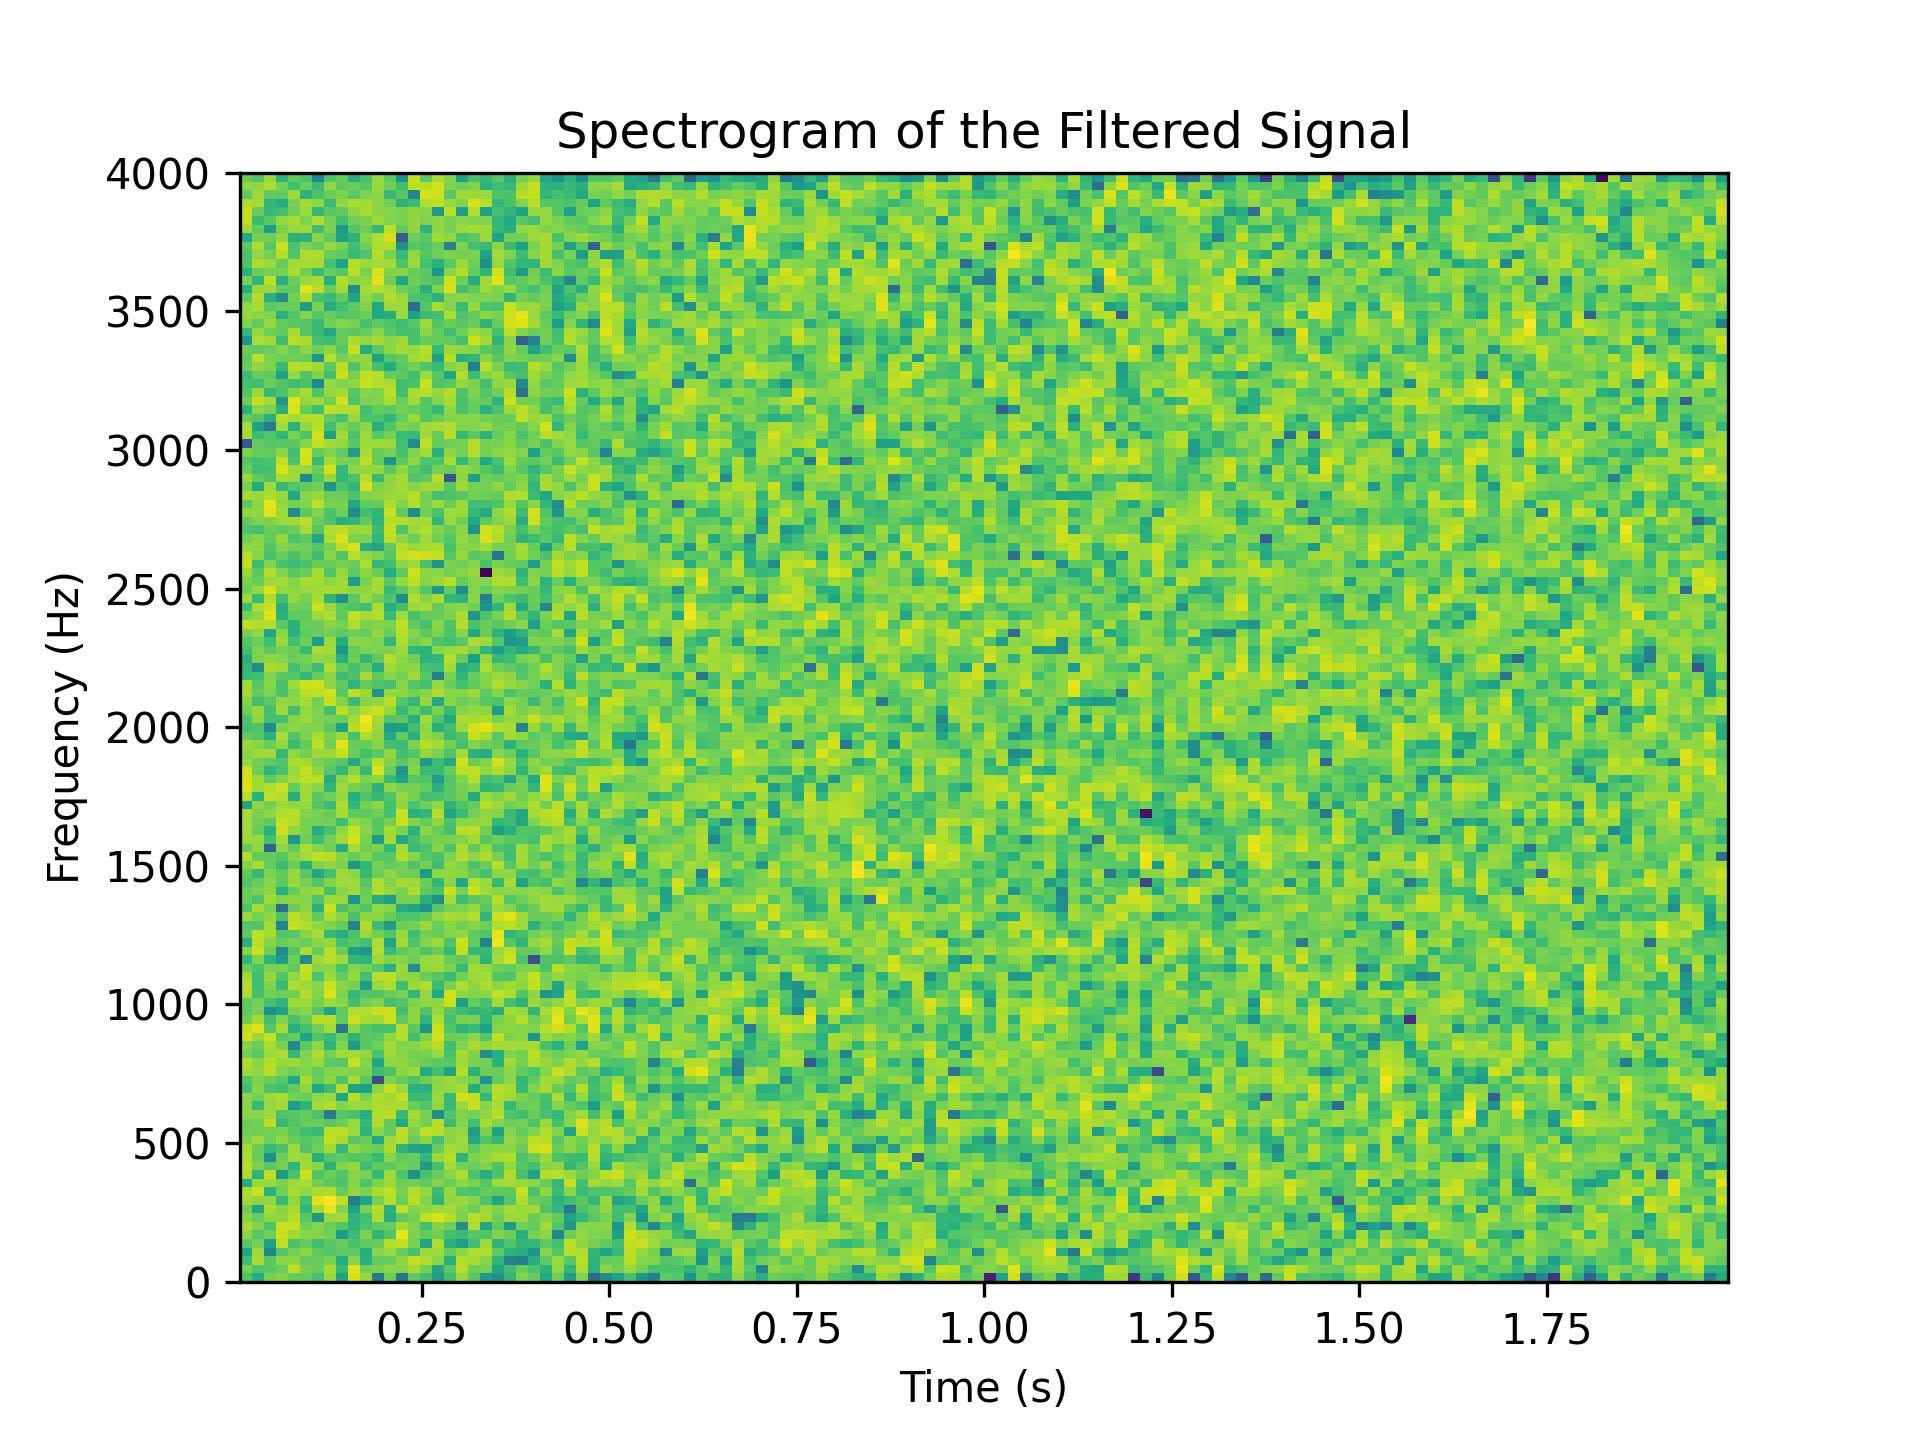
\includegraphics[width=\linewidth]{images/spectrogram_output_c_9.png}
    \end{minipage}\hfill
    \caption{Spectrogram of $2^{nd}$ order ANF with $\lambda = 0.9$ in C(left) and Assembler(right)}
    \label{fig:adaptive_c_spectrogram_l9}
\end{figure}



The setting of $\lambda = 0.9$  demonstrates significant noise reduction at 400 Hz and 1200 Hz. Comparable results from a C implementation (\autoref{fig:adaptive_c_spectrogram_l9}) were also presented .


For intuitive comparison, we plot the frequency responses of the input and the output signals from the ANF in both assembly and C (\autoref{fig:input_frequency_response}, \autoref{fig:adaptive_frequency_response}). These plots underscore the Adaptive $\rho$ mechanism, enhancing the convergence speed and tracking ability of the filter.

\begin{figure}[ht]
\centering
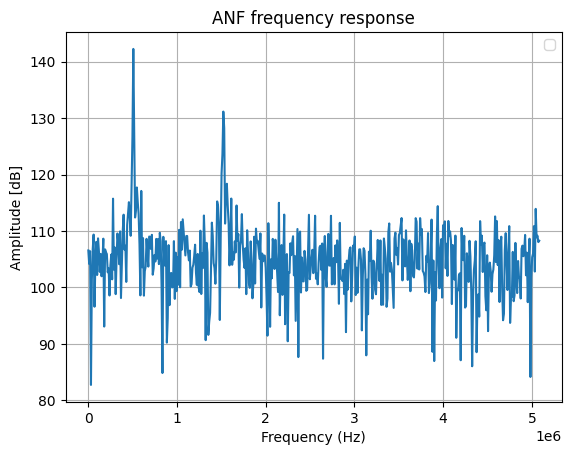
\includegraphics[width=0.5\columnwidth]{images/input_frequency_response.png}
\caption{Input frequency response}
\label{fig:input_frequency_response}
\end{figure}

Comparatively, the frequency responses after filtering (\autoref{fig:adaptive_frequency_response}) show the effective removal of the narrow band and high intensity frequency components at 400Hz and 1200Hz.

\begin{figure}[ht]
    \centering
    % First figure
    \begin{minipage}{0.475\columnwidth}
        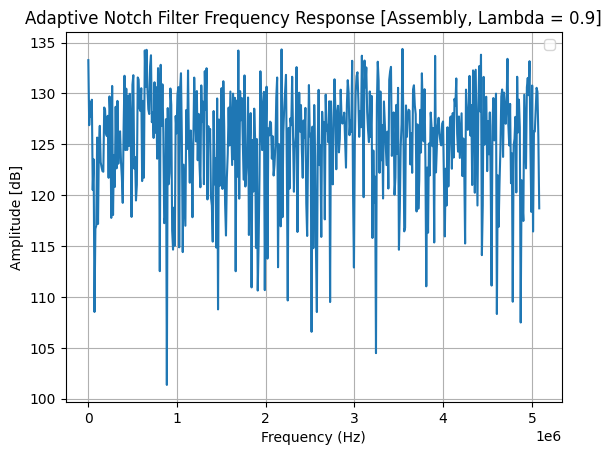
\includegraphics[width=\linewidth]{images/Adaptive_Notch_Filter_Assy_Frequency_Response_L9.png}
    \end{minipage}\hfill
    % Second figure
    \begin{minipage}{0.475\columnwidth}
        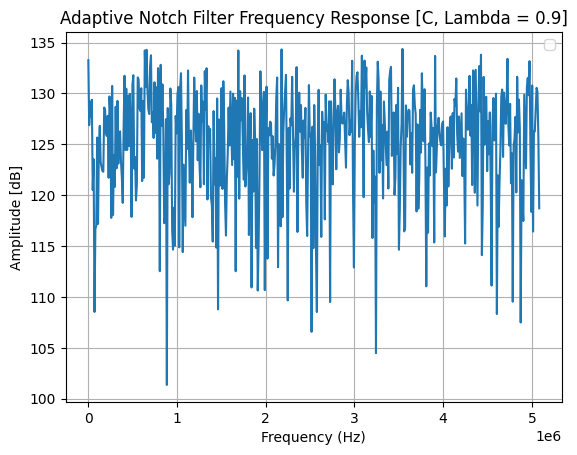
\includegraphics[width=\linewidth]{images/Adaptive_Notch_Filter_C_Frequency_Response.png}
    \end{minipage}\hfill
    \caption{Frequency Response of ANF with adaptive $\rho$ and $\lambda = 0.9$ in C(left) and Assembler(right)}
    \label{fig:adaptive_frequency_response}
\end{figure}


\subsection{Computational cost analysis}
The computational efficiency of our ANF implementations was quantified in terms of clock cycles, a direct measure of processing time. The results, as detailed in Table \ref{tab:comp_cost}, indicate that both the C and Assembler implementations have similar computational demands. This similarity suggests that our optimization strategies were effective across both programming languages, maintaining a balance between performance and computational resource utilization. 

However, it is noteworthy that even minor differences in clock cycles can have significant implications in resource-constrained environments. Therefore, future work will focus on further optimizing the computational efficiency of our ANF, particularly for deployment in embedded systems or platforms with stringent resource limitations.


\begin{table}[ht]
\centering
\begin{tabular}{l|l}
\hline
Implementation                     & Clock cycle \\ \hline
ANF with $\lambda = 0.9$ in C         & 16,733,840  \\
ANF with $\lambda = 0.9$ in Assembler & 16,733,632  \\
ANF with $\lambda = 0.9$ in C         & 16,733,519  \\
ANF with $\lambda = 0.9$ in Assembler & 16,733,377 \\ \hline
\end{tabular}
\caption{Computational cost (clock cycles) of all different implementation}
\label{tab:comp_cost}
\end{table}



\clearpage

%
% ---- Discussion ----
%
\section{Discussion}
\subsection{Implementation evaluation}
In our project, the adaptive notch filter (ANF) demonstrated substantial noise reduction capabilities, specifically at target frequencies of 400 Hz and 1200 Hz. The spectrogram analyses clearly illustrated the attenuation of these frequencies, validating the effectiveness of our ANF design in noise component removal. Moreover, the incorporation of an adaptive $\rho$ value not only added flexibility to the filter's response but also potentially enhanced its convergence speed and tracking ability, making it more suitable for dynamic signal environments.

\subsection{Computational Efficiency}
Another critical aspect for practical applications is the computational efficiency of the ANF implementation on the TMS320C5515 platform. While the clock cycles resources utilization were evaluated, memory exploitation and the trade-off relatoinship between speed and memory usage were not evaluated. Such measruements would enable a informed program development and configuration selection based on applications. 

\subsection{Choice of fixed-point Q-factor for each variable}
The current Q-format choice for $s$ is $16q11$, yet after re-evaluation, the Q format for $s$ can be set to $16q12$ given only three integer bits are needed. The one more fractional bits would allow a more precised computation.

\subsection{Future Work}
Moving forward, our research will focus on analyzing the trade-offs inherent in noise reduction, signal distortion, and computational efficiency. We aim to thoroughly explain the rationale behind the design choices in our ANF and the quantization scheme employed. Addressing the challenges encountered during the implementation phase will also be a key area of our future work. Additionally, we plan to explore potential directions for further research and improvements to enhance the filter's performance and applicability in various real-world scenarios.

For objective performance evaluation, Mean Log-Spectral Signal Distortion (SD) will be employed, as referenced in \cite{5675660}. SD is a quantitative measure of sound quality, assessing distortion introduced by notch filters and howling phenomena. The mathematical formulation of SD is given by:
\begin{equation}
SD(t) = \sqrt{\int_0^{f_s / 2} \left(10 \log_{10} \frac{S_y(f)}{S_x(f)}\right)^2 df}
\end{equation}
where \( S_x(f) \) and \( S_y(f) \) represent the power spectral densities of the original and filtered signals, respectively, and \( f_s \) is the sampling frequency.



\clearpage

%
% ---- Bibliography ----
%
% Add your references to the file 'mybibliography.bib'. Then cite the references with the following command: \cite.
%
% BibTeX users should specify bibliography style 'splncs04'.
% References will then be sorted and formatted in the correct style.
%
\bibliographystyle{splncs04}
\bibliography{mybibliography} \label{references}
%

\end{document}
